%!TEX program = xelatex

\documentclass{HustGraduPaper}
\title{移动网络数据挖掘的研究与应用}
\author{徐聪}
\date{\today}
\school{电子信息与通信学院}
\classnum{通信1403班}
\stunum{U201413500}
\instructor{王邦}

\begin{document}
    \maketitle
    \statement
    \clearpage
    \pagenumbering{Roman}

    \begin{cnabstract}{移动网络;数据挖掘;统计分析}
        这里是摘要内容。
    \end{cnabstract}
    \begin{enabstract}{Mobile network;Data mining;statistic analysis}
        Here is the content of abstract.
    \end{enabstract}

    \tableofcontents
    \clearpage
    \pagenumbering{arabic}

    \section{绪论}
    
    \subsection{选题背景与意义}

    随着我国进入经济社会高速发展的阶段,电信行业也得到了快速的发展。从上世纪九十年代的
    2G发展落后于世界;到本世纪初3G时代,由我国大唐电信主导提出的TD-SCDMA标准被ITU确立成为3G主流
    制式;进入4G时代后,我国发展时间轴基本与世界先进水平国家保持同步,由我国主导的 TDD 通信制式
    将成为 5G 主流制式。到了 5G时代,我国主动成立 IMT-2020 推进组,积极推进 5G 技术标准发展,有望实现技术与市场双引领。
    
    除了传统通信的2、3、4G通信网络,中国的电信运营商也在顺应移动互联网发展趋势,
    发展出了诸如IPTV、窄带物联网(NB-IoT)等新兴业务。以一个三线城市市级运营商来说,
    其网络管理中心负责主要业务包含无线及有线总共十二类业务,支撑十二类业务的背后包含十三类网络、四大类设备。
    如此众多的业务伴随而来的是海量的数据:日志、参数、拓扑等等。

    面对如此海量的数据,网络维护管理人员的维护难度也在不断攀升。传统的电信网络维护管理方式通常是以人工管理为主,
    运营商会向提供技术支持的公司雇佣代维人员对网络进行代理维护,而运营商内部人员则注重于对网络的管理以及自身核心业务,
    这种代维模式最初是为了解决网络规模扩张、运营商间的竞争压力不断增大的问题。但随着数据网络规模的进一步扩大,网络复杂性呈
    指数型上升,但是代维人员规模却不可能同步增加。除此之外,由于代维行业没有统一的行业标准,会出现代维人员业务水平参差不齐
    的情况,且在日常维护工作中仍采取较为传统的手段,导致运营商对于网络的管理维护并没有跟上网络快速发展的步伐,传统的维护
    模式已经不能适应未来的需求。

    近年来,随着计算能力的提升以及信息技术的发展,大数据的概念在运营商对网络管理维护中得到了广泛传播,将大数据以及数据挖掘的技术
    引入对于电信网络的运维管理来说是解决当困难及满足未来需求的一种手段。由于运营商的特性,导致了它在数据规模这一块拥有
    天然的优势,而当前运营商的问题也是由于数据量过于巨大,而自身管理手段跟不上增长速度,导致的运维管理难度上升,
    而大数据及数据挖掘技术的引入会将这一劣势变为优势,不仅能解决当前数据量过大无法处理的难题,还能在此基础上对整个网络的流量、设备以及业务进行集中管控、统一编排。
    同时近年随着人工智能概念的火爆,一定程度上也是基于大数据及数据挖掘技术的成熟,因此在对电信网络数据进行大数据管理以及数据挖掘的基础上可以在合适的场景引入
    人工智能的方法,实现面向未来的智能运维。
    
    综上所述,移动通信网络的数据挖掘对于提升整个网络运维管理效率及质量具有较为实际以及深远的意义。在实际研究过程中,对运营商而言,数据挖掘意味着需要大数据,而
    大数据意味着对数据的获取、存储、分析、呈现等方式都提出了新的挑战,因此,如何对传统运维方式的这几个方面进行革新成为了建设大数据系统,从而实现对数据的深层价值挖掘的
    关键点。与此同时,运营商也希望通过这一举措,将复杂的网络进行高效的管理,这对于提升用户感知、网络优化、网络规划等多方面都具有实际的意义。\\
    \begin{generalfig}[htb]{大数据信息处理框架}{fig:frame}
		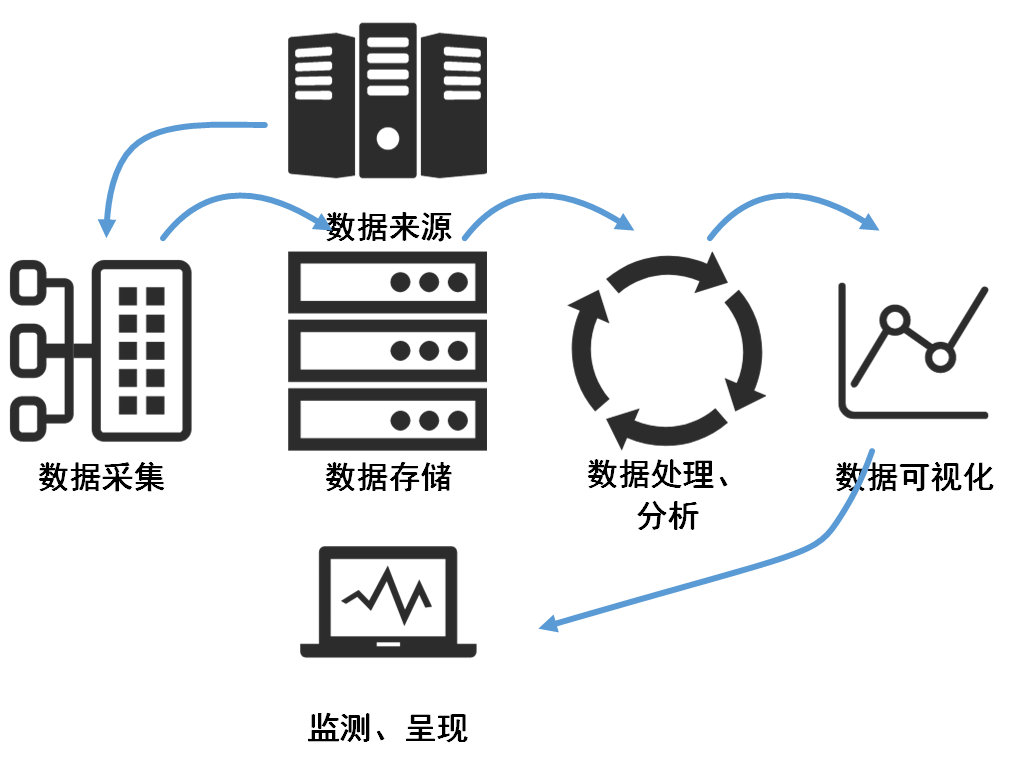
\includegraphics[width=\textwidth,scale = 0.5]{Figures/frame.png}
	\end{generalfig}

    \subsection{论文内容与成果}

    本文就数据挖掘技术在运营商网络管理和分析中的可行性应用展开探索性讨论,从运营商现状出发,结合实际情况以及运维中的痛点进行分析,提出建设大数据系统应用数据挖掘技术解决运维难题是未来的趋势这一观点,并由此
    利用建设大数据系统的方法尝试解决运营商面临的海量数据的采集及处理问题,同时还在大数据系统的基础上运用数据挖掘技术解决运维难题进行了初步的尝试。
    主要内容分为三个部分:

    第一部分就当前运营商面临的多系统数据采集的难点进行探索解决,由于运营商对网络情况感知的实时性要求较高,因此提出采用主动监控的方式采集数据并在采集数据后对数据进行预处理及存储,
    为上层的分析和应用提供数据基础,同时针对运营商的多系统多数据源这一现状这里提出采用区别于传统采集手段的分布式采集系统。

    第二部分在采集模块采集预处理存储后的数据基础上进行分析,尝试从价值密度较低的数据中挖掘出对运营商网络管理有利的结论或建议。具体来说,本文就网络情况监控中的KPI异常检测问题进行了分析,
    并提出了利用数据挖掘来解决问题的一种思路。

    最后,第三部分的数据呈现部分本文提出采用丰富的图表形式来对数据分析结果进行直观有效的展示,使得网络管理运维人员能够更加清晰直观地了解网络情况,能对网络问题及时做出应对。

    \subsection{论文结构}

    第一章绪论,主要介绍论文的选题背景以及研究意义,介绍了当前运营商在网络管理维护工作中的窘境,由此提出运用大数据以及数据挖掘技术在相关工作中
    的作用以及意义,随后对本文所作的工作进行了简要的介绍。最后介绍了本篇文章的组织架构。

    第二章相关知识综述,对运营商的网络现状进行了介绍,介绍了运营商的网络数据管理现状;还对建设大数据系统地相关技术知识进行了概述,包括了数据采集、数据存储、数据呈现方式,
    为实际的探索应用确立了思路与基础。

    第三章为移动网络数据挖掘应用的设计与实现,包括对系统的需求分析、系统架构以及部分功能的设计及实现,包括了数据采集、数据呈现。本章还就如何利用大数据系统进行在异常检测问题上使用数据挖掘方法进行了初步的探索。

    第四章为总结与展望,主要对本文所作工作进行总结,总结本文的创新点以及在实际应用中的意义,同时指出设计上的不足,为未来的工作方向做出展望。

    \clearpage
    \section{相关知识综述}

    \subsection{运营商网络运维现状介绍}

    现在是一个数据化的时代,也是一个移动化的时代。著名分析公司Gartner在报告中指出未来的公司都将是数据公司,现代人生活中被各种移动应用所环绕,移动网络流量
    出现井喷式的增长。作为网络运营商来说,爆炸增长的数据流量意味着网络管理维护难度的升级,更为重要的是,如果在数据时代不能完成运营商自身的定位转型,会使得自身逐渐管道化最终失去活力与竞争力,
    因此如何避免自己逐渐代边缘化是当前时代环境下运营商所面临的挑战。但随着大数据及数据挖掘技术的成熟,上文所提到的挑战也可以转化为运营商转型升级的机遇,
    如何在保证自己服务质量的同时,发挥天然具有的流量数据优势,无论是从海量的日志数据中分析出网络问题的根源,还是从流量数据中挖掘出具有经济、商业、政治意义的有效结论,都对运营商增强自己的竞争
    能力、避免边缘化、完成IT化转型升级具有重要的战略意义。

    目前部分运营商对网络的管理存在这以下几个方面的问题:数据来源多样化:与传统的数据来源较为单一不同,由于现在运营商的业务扩展,所以不同业务的数据存放的服务器也不同,
    单一的数据来源可以依靠人工或者简单的采集脚本进行采集,但是数据来源增加后,传统的方法就显得低效和不可行了,此外数据量的增加也对数据采集的实时性提出了更高的要求;
    数据分析浅层化:运营商虽然拥有海量的数据,但是传统的分析方式只注重于简单的统计,难以从价值密度较低的数据中挖掘深层关联以及结论;数据呈现单一化:目前部分运营商的网络运维
    是交给代维人员进行代理维护的,由于缺乏统一的行业标准,代维人员水平参差不齐,导致最后结果的呈现形式较为原始和不直观,对于专业知识不够全面的但同时关注网络状况的人
    (领导层)来说,无法快速了解网络情况。

    目前中国移动、中国电信、中国联通三大运营商均加速了自己的大数据平台建设,旨在发挥自身数据价值,利用数据挖掘技术将数据优势转化成大数据周边服务,对于运营商提升用户感知、提高管理效率、
    增强流量化经营都起到促进作用。除此之外,各地市级运营商也在积极与高校进行合作,在提升自身技术水平的同时也推动了学术研究的进展,对于科技的进步也具有着重要的意义。
    与此同时,国外的运营商们也早早开始了大数据建设:美国第二大电信运营商AT\&T收集了用户的位置信息并通过数据挖掘技术对用户行为进行分析,并将其数据打包出售给广告公司以达到
    精准营销的目的;法国电信根据用户消费行为进行分析,同时结合通话投诉情况对网络结构进行优化;韩国通讯社SK新成立一家公司专门处理大数据业务,目标是提升客户感知,实现精准化
    营销。

    \subsection{数据挖掘相关技术概述}
    近年来,随着人工智能、机器学习概念的火爆,数据挖掘这一词汇又重新进入了人们的视野。数据挖掘是指运用人工智能、机器学习、统计学和数据库的交叉方法在海量数据中发现特定模式或规律结论的过程。
    数据挖掘过程的总体目标是从一个数据集中提取信息,并将其转换成可理解的结构,以进一步使用。除了原始分析步骤,它还涉及到数据库和数据管理方面、数据预处理、模型与推断方面考量、兴趣度度量、
    复杂度的考虑,以及发现结构、可视化及在线更新等后处理。而将数据挖掘技术引入到运营商的网络管理维护中来这一想法符合当下技术发展的潮流,也符合运营商自身发展的需求。
    
    数据挖掘过程往往伴随着数据采集、数据预处理、数据存储、数据分析、数据呈现等几个关键步骤,其中数据采集、数据存储、数据呈现都是建设大数据系统所需要的技术,所以下文就
    数据采集、数据存储以及数据呈现方式进行简要概述。
    \subsubsection{大数据采集技术概述}
    
    如\autoref{fig:frame}所示,数据采集是所有大数据应用中不可或缺的一部分,特别是在运营商本身具有多种业务系统的情况下,数据采集的挑战也变得尤为突出,其中主要包括:
    \begin{itemize}
		\item 数据源的多样性
        \item 数据量的规模大、实时性要求高
        \item 对采集可靠性的保证
        \item 避免重复数据
        \item 保证采集质量
    \end{itemize}
    为了应对以上的挑战,传统的单一采集必然不能满足需求,现如今各种大数据采集技术都选用分布式采集方式,如Apache Flume、Splunk Forwarder等,这些工具都是去中心化,同时能够保证
    数据采集的实时性和有效性,能够较好的满足大数据采集需求,下面分别介绍这两种常用的数据采集技术。
    \bigskip
    {\songti \bfseries Apache Flume\\}

    Flume是Apache旗下的一款开源的、高可靠、可扩展、易管理的分布式数据采集系统,除此之外 Flume还具有数据预处理功能。Flume使用JRuby构建,所以需要依赖JAVA环境。Flume最初是由Cloudera的工程师开发出来想用于
    合并日志数据的分布式系统,但随着时间的发展以及大数据趋势的来临,使得Flume逐渐发展成为了用于处理流数据事件的常用系统工具。%\cite{备注}。

    \ Flume的设计是由一个一个的代理(agent)组成的代理网络作为管道,管道两端分别是数据源和目的地。每一个agent由采集器(Source)、传输通道(Channel)、及注入器(Sink)组成。
    采集器负责接收输入数据并将数据送入传输通道;传输通道主要作用是对数据进行缓存,在传输给注入器之前对数据进行缓存,缓存方式可以根据配置文件配置成内存、文件、JDBC等;
    注入器的作用是将数据从传输通道钟读取出来,随后发送给下一个代理或最终目的地(存储空间)。Flume在每一个agent的采集器端和注入器端都采取了transaction的机制,保证信息传输
    安全稳定,同时Flume支持故障转移(failover)和负载均衡(load balance),当某个agent失效时并不会影响整体系统运行,这也确保了系统运行的稳定和可靠性。

    \begin{generalfig}{Flume组织架构}{fig:flume}
        \includegraphics[width=\textwidth]{Figures/flume.png}
    \end{generalfig}
    {\songti \bfseries Splunk Forwarder\\}
    
    与上文所提到Flume的开源性不同的是,Splunk作为商业化公司所提供的完整数据采集、数据分析、数据呈现的一整套解决方案。这个方案中包含三个部分:Search Head负责数据的搜索和处理;indexer负责创建数据的索引
    与数据的存储;Forwarder负责数据的收集、清洗变形并发送给indexer。Splunk内置了对Syslog,TCP/UDP,Spooling的支持,同时,用户可以通过开发Script Input和Modular Input的方式来获取特定的数据。
    在Splunk提供的软件仓库里有很多成熟的数据采集应用,例如AWS,数据库(DBConnect)等等,可以方便的从云或者是数据库中获取数据进入Splunk的数据平台做分析,同时Forwarder也支持负载均衡。
    
    \begin{generalfig}[htb]{Splunk组织架构}{fig:splunk} 
        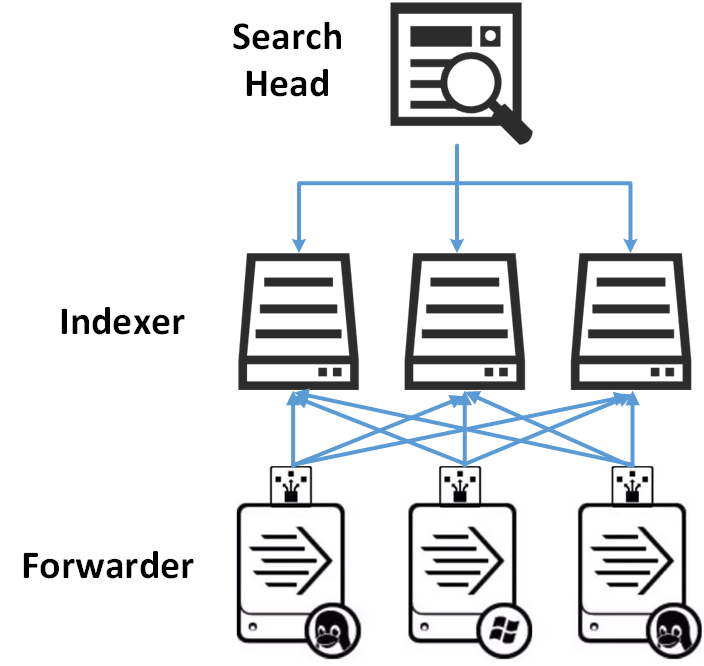
\includegraphics[scale = 0.4]{Figures/splunk.png}
    \end{generalfig}

    \subsubsection{大数据存储技术概述}
    大数据场景下,传统的存储技术已经不能满足海量的数据存储以及高频率的查询与存储,同时对于数据挖掘技术来说,传统的关系型数据库也无法满足复杂的关联分析等需求,除此之外,大容量的存储设备即使有着摩尔定律的
    存在,对于满足大数据要求的存储器价格仍然十分高昂。如此众多的情况与困难下,分布式存储似乎成为了当前环境下建设大数据系统的唯一也是最好选择。下面介绍一种强大的分关系型数据库集群:\\
    {\songti \bfseries GreenPlum\\}
    GREENPLUM是一个关系型数据库集群. 是由多个独立的数据库服务组合而成的逻辑数据库。与RAC不同,这种数据库集群采取的是MPP(Massive Parallel Processing 即大规模并行处理)架构。如下图所示

    \begin{generalfig}[htb]{GreenPlum架构}{fig:GreenPlum} 
        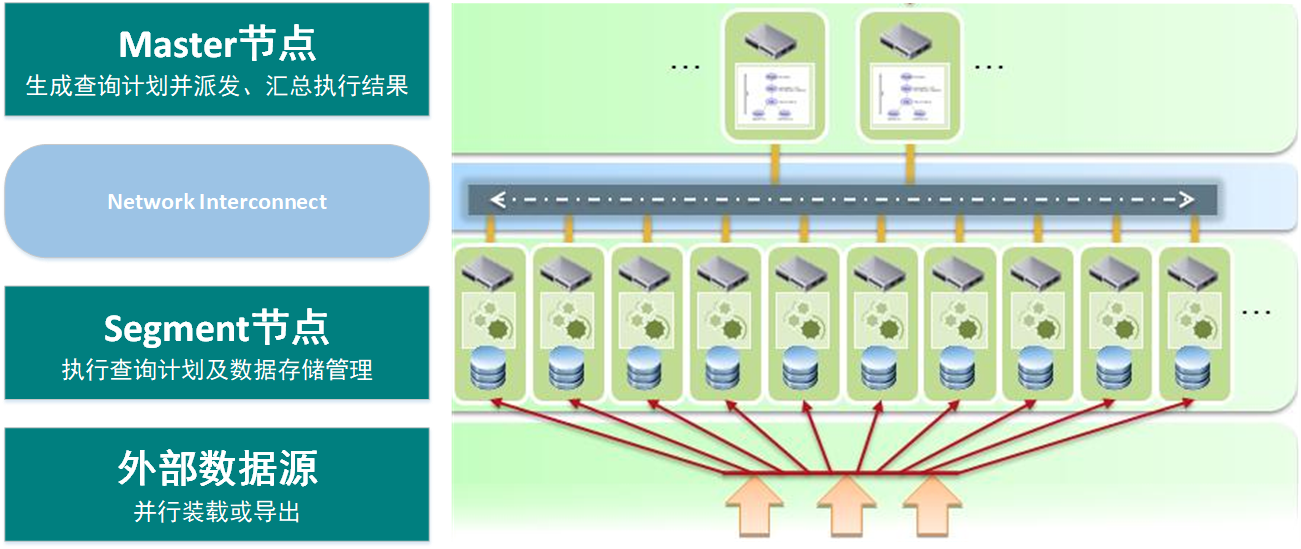
\includegraphics[width = \textwidth]{Figures/GreenPlum.png}
    \end{generalfig}

    它的组件分成三个部分MASTER节点、SEGMENT节点以及MASTER与SEGMENT之间的高效互联技术GNET。其中MASTER和SEGMENT本身就是独立的数据库服务器。不同之处在于,MASTER只负责应用的连接,生成并拆分执行计划,
    把执行计划分配给SEGMENT节点,以及返回最终结果给应用,它只存储一些数据库的元数据,不负责运算,因此不会成为系统性能的瓶颈。这也是GREENPLUM与传统MPP架构数据库的一个重要区别。 
    SEGMENT节点存储用户的业务数据,并根据得到执行计划,负责处理业务数据。也就是用户关系表的数据会打散分布到每个SEGMENGT节点。当进行数据访问时,首先所有SEGMENT并行处理与自己有关的数据,
    如果需要segment可以通过进行innterconnect进行彼此的数据交互。 segment节点越多,数据就会打的越散,处理速度就越快。因此与SHARE ALL数据库集群不同,通过增加SEGMENT节点服务器的数量,
    GREENPLUM的性能会成线性增长。优点是查询速度快、数据装载快,且拥有非常好的可扩展性。

    \subsubsection{大数据呈现技术概述}
    在运营商日常的网络管理工作中,会有各种各样的报表制作需求,从简单的每日流量统计情况、到每月网络整体情况总结,亦或是突发故障分析报告,都离不开数据的呈现与展示。但现阶段在部分运营商的报表制作
    呈现中,由于时间和技术的限制,往往还充斥着较为原始的数据罗列和单一的折线表现形式,这种表现形式除了制作者能对其中的含义能够快速清晰的了解,由于报表呈现展示的对象通常是不具备全面专业
    知识的管理者,这些信息对他们来说不够直观清晰,理解起来较为费劲,遇见突发状况时也不能对网络情况快速做出应对,导致客户感知较差,网络管理效率较低。因此,在日常报表制作中将数据转化成
    清晰直观恰当的图标形式会使得数据呈现效果大幅提升。接下来就现在常用的一种数据呈现工具进行简要介绍:

    {\songti \bfseries FineBI工具\\}

    FineBI 提供强大的可视化图表,表格以及过滤组件,用户只需在 dashboard面板中简单拖拽操作,便能制作出丰富多样的数据可视化信息,并可以进行数据钻取,联动和过滤操作,自由地对管理过程中产生的数据进行分析和探索。
    该工具还提出了极具实用价值的业务数据包概念,借助业务数据包我们可以轻松实现按照业务对数据进行分类、管理和权限配置。业务数据包是 FineBI 多维数据库在前端的映射,通过业务包的创建和设置,使得多维数据库和业务分析需求的衔接更加紧密自然。
    \begin{generalfig}[htb]{FineBI}{fig:FineBI} 
        
\includegraphics[scale = 0.4]{Figures/FineBI.png}
    \end{generalfig}

    \subsection{本章小结}
    本章对关于数据挖掘在移动网络管理中的应用的相关设计技术以及运营商网络管理运维现状进行了较为概要的阐述。首先从当前运营商在移动网络时代对于自身定位以及
    网络管理上遇到的窘境进行了描述,随后指出了传统运维的不足以及对国内外运营商针对大数据和数据挖掘所做的工作进行了简介。然后对应用于大数据和数据挖掘技术的分布式
    数据采集技术以及数据呈现方式进行了较为详细的描述,为第三章的应用设计和实现做好技术准备。
    \clearpage

    \section{移动网络数据挖掘应用的设计与实现}
    \subsection{系统需求分析与设计}
    某市级运营商网络管理中心的主要功能职责包括对整个市区内的网络设备、业务、通信网络、用户服务等提供维护保障,目前包括十二类业务,业务规模包括有线业务和无线业务;除此之外还包括
    对四大类设备的维护,分别是交换设备、数通设备、传输设备、动力设备,四大类设备下还包括各种专业设备;网络部分分为专业网与支撑网两大类共十三类网络。如此众多的维护对象,每天处理的数据
    量必然是无比庞大的,因此需要一个大数据系统能够自动采集各类数据并进行分类存储,以供上层大数据应用分析使用,最后以直观的形式进行反馈输出。

    \begin{generalfig}{十三类网络}{fig:Networks} 
        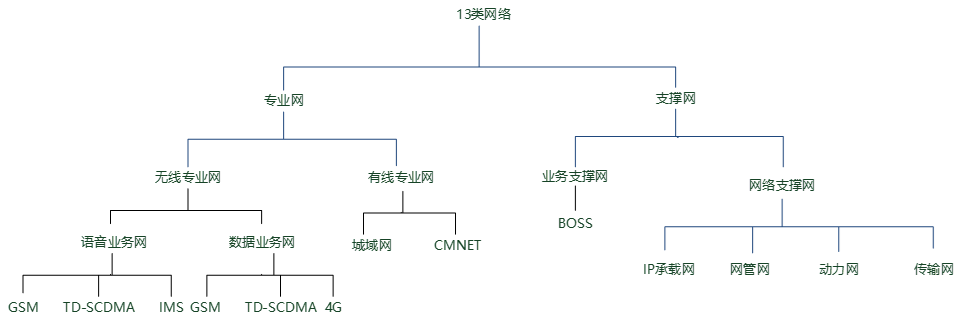
\includegraphics[width = \textwidth]{Figures/networks.png}
    \end{generalfig}

    由于具体数据应用分析需要结合具体需求以及数据特性定制,而本文进行的只是利用建设大数据系统从而为在运营商的网络运维管理上运用数据挖掘技术的尝试性探索,并不能直接拿到数据和需求进行算法设计,因此本文的重点在于需求分析以及
    数据采集模块以及数据呈现模块的设计,关于进一步的对数据的分析利用,仅进行简单的举例说明。
    \subsubsection{数据源分布介绍}
    运营商内部目前存在多个管理系统,运维人员在执行不同的运维任务时需要通过登陆不同的系统服务器进行数据下载,但是实际分析过程中可能会用到多方数据,由此挖掘数据之间潜在的关联性和规律性。单以十三类网络中的城域网
    日常运维工作举例,需要用到的数据类型和对应系统如下表所示:

    \begin{generaltab}{城域网维护工作所需数据及来源}{tab:heightweight}
		\begin{tabularx}{\textwidth}{lCCC}
			\toprule
			数据类型&来源\\
			\midrule
			家宽、IPTV等业务在线人数&本地管理系统\\
			端口流量利用率&省公司网管系统\\
			IPTV地址池利用率&省公司信息系统\\
			互联互通流量数据&流量分析系统\\
			.... & ....\\
			\bottomrule
		\end{tabularx}
    \end{generaltab}
     
    上表只列举了部分数据来源及系统,其中本地管理系统及流量分析系统都属于本地系统,本地系统只与本地的部分设备相连,因此本地系统的数据是不全面的,而省公司网管系统和省公司信息系统服务器架设在省公司机房,
    这些系统跟本地所有设备相连。各级系统的组织架构如下图所示:

    \begin{generalfig}{各级系统组织结构}{fig:SJYJG} 
        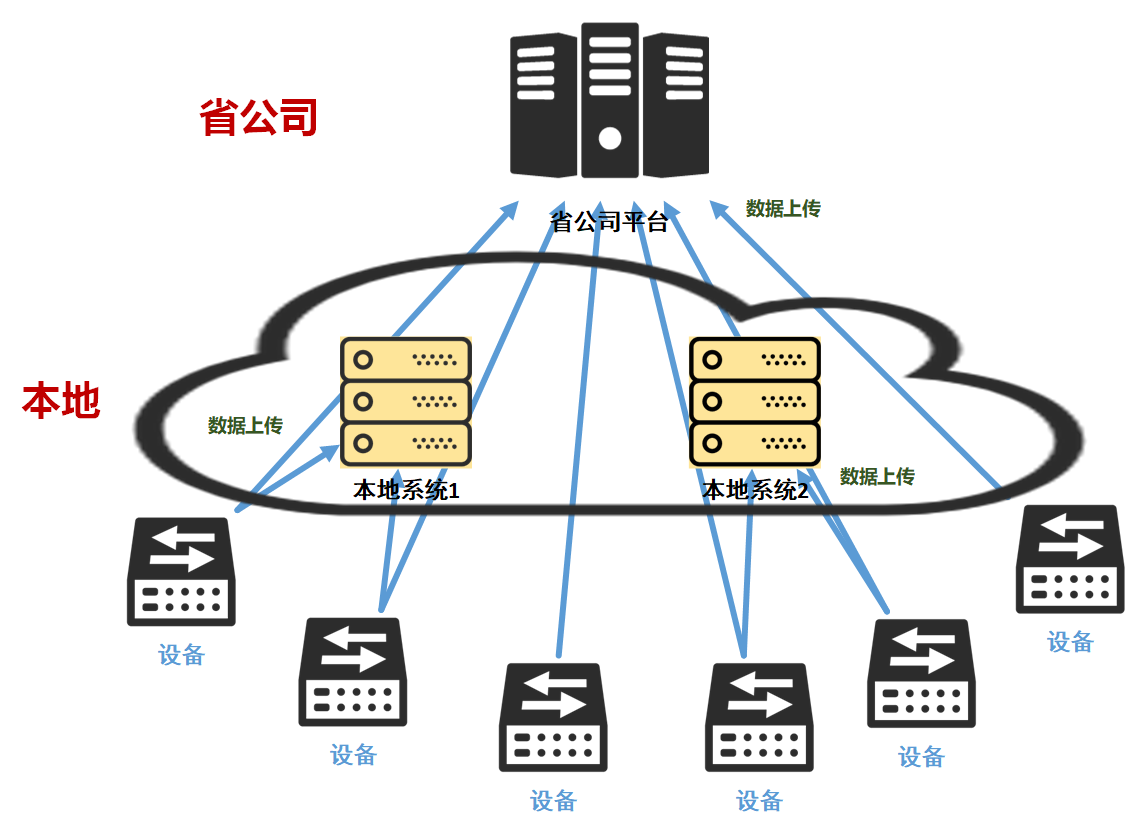
\includegraphics[width = \textwidth]{Figures/SJYJG.png} 
    \end{generalfig}

    \subsubsection{系统需求分析}
    本文就运营商大数据系统的设计和实现进行探索和可行性分析,该系统实现后,从数据上能够自动采集本地所有与网络维护管理有关的数据,从而实现对数据的本地化、统一化管理,缩短了重复登陆系统获取数据的时间;
    从业务上来看,通过对采集的数据进行数据挖掘和分析,能够更好的掌握客户行为意义与兴趣,挖掘数据背后潜在的商业价值,提升客户感知,从而达到提升业务满意度的目标;从网络维护来看,通过对采集的日志信息进行
    分析,利用成熟的算法对网络故障进行根因分析和故障定位辅助,给出故障排查或网络优化的建议。

    综上所述,该系统应当满足如下需求:

    (1) 具有后台自动对全网数据的采集、预处理、存储能力。由于移动业务正处于快速发展时期,未来更多业务会涌现而出,因此采集能力需要具有一定扩展性,以面向未来的业务发展;除此之外,为了得到高质量和可靠有效的数据
    进行数据分析,系统还需具有对采集数据的一定预处理能力,为将来的数据分析应用提供坚实的基础。
    
    (2) 具有良好的数据呈现界面,由于数据量过于庞大,采用传统的数据罗列和文字总结会使得使用人员过于疲劳从而无法快速了解情况,因此数据呈现部分需要具备良好的视觉呈现效果,使得重点突出、一目了然。对于不同类型
    的数据呈现的侧重点不同,表现形式应当也随之而变化,即使是不具备专业知识的人也能一眼看懂。
    \subsubsection{系统整体设计}
    通过系统第二章关于数据采集、数据存储、数据呈现等知识的概述以及上一节对于系统需求的分析,结合这两方面的知识从工程实现角度给出如下系统结构:
    \clearpage
    \begin{generalfig}{系统架构}{fig:XTJG} 
        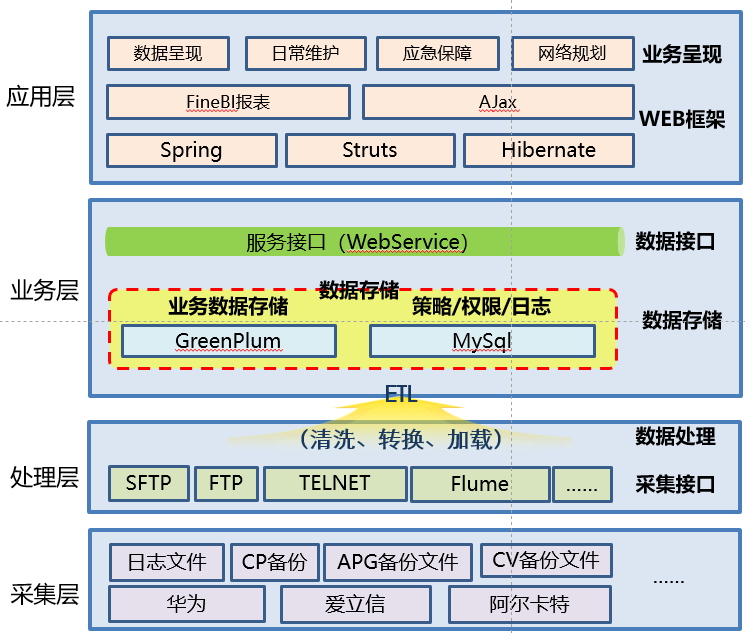
\includegraphics[scale = 0.7]{Figures/XTJG.png} 
    \end{generalfig}
    
    其中处理层提供SFTP$\backslash$ FTP$\backslash$ TELNET$\backslash$ SNMP等多种实时$\backslash$非实时的采集方式,这些采集方式用于在未连接到服务器上的设备中进行数据采集,同时也为了采集某些不常用的数据,
    而前文提到的Flume技术就从已有系统的服务器上进行日志、数据采集,同时这两种方式都留有一定扩展性。

    通过处理层采集的数据进行清洗、转换、加载后根据数据类型分别采用GreenPlum 和 Mysql两种方式进行存储,其中GreenPlum用于存储业务指标数据,MySql用于存储任务策略、权限、日志等数据。

    上层应用层通过数据接口调用数据进行网络维护工作的支撑,其中数据呈现部分通过ajax对数据进行实时更新以及FineBI软件进行前端呈现。

    以上是作者对于一个成熟的大数据系统的设想以及在实现的路上的探索,{\songti \bfseries 但是由于能力和时间约束,仅对其中部分功能进行了模拟实现},因此接下来就其中的数据采集及存储部分、数据呈现部分的设计与实现进行简要描述。
    \subsection{数据采集及存储部分的设计与实现}
    \subsubsection{具体需求分析}
    本部分包含数据采集以及数据存储两部分的需求分析,接下来对两个方面分别进行描述:
    
    (1)本如果要搭建一个大数据系统,采集数据的方式有两种:编写采集脚本直接通过传统手段(如FTP,SFTP等)从相应设备上取,这种方式的好处是能够比较直接的取到任何想要取得的数据,但是缺点是较为低效;另一种方法是
    在已有的系统服务器上进行分布式采集系统的部署,通过采集系统对服务器进行监控并设置采集粒度进行自动采集,这种方式的优点是能够较为高效的进行数据采集,缺点是对于没有链接到系统服务器的设备上的数据无法进行采集。
    
    结合案例中运营商的实际情况,设计的数据采集功能应该满足从多数据源进行数据采集,同时保有一定扩展性以满足将来业务的扩张需求,同时还需要尽可能地多支持不同类型数据的采集。

    (2)对于数据存储功能的需求就相对简单了,对于大量、高频的数据来说,存储的要求是快速、具有可靠的并发性;而对于相对来说采集较为低频但是查询较为频繁的数据(如日志文件),希望能够达到快速查询和易用性的要求。
    \subsubsection{设计与实现}
    根据前文对数据采集以及数据存储的功能需求分析,结合第二章中对相应技术的介绍,我们最终选择:

    {\songti \bfseries-对于数据采集功能:}
    
    选用Flume分布式采集系统与传统采集系统并用的方式:传统采集方式通过编写脚本文件通过不同协议登陆设备进行采集;而Flume采集的方式则是在已有已有系统的服务器上部署Flume,通过多个agent进行文件的采集,
    每一个agent对一个目录下的文件进行监控和采集,一旦监控下的目录出现新的数据,agent则立即进行采集上传,通过配置agent-collector完成对数据的汇总,然后通过flume自带的预处理工具进行清洗后存入相应的存储位置。
    架构大致如下图所示:
    \clearpage
    \begin{generalfig}{数据采集功能架构}{fig:SJCJJG} 
        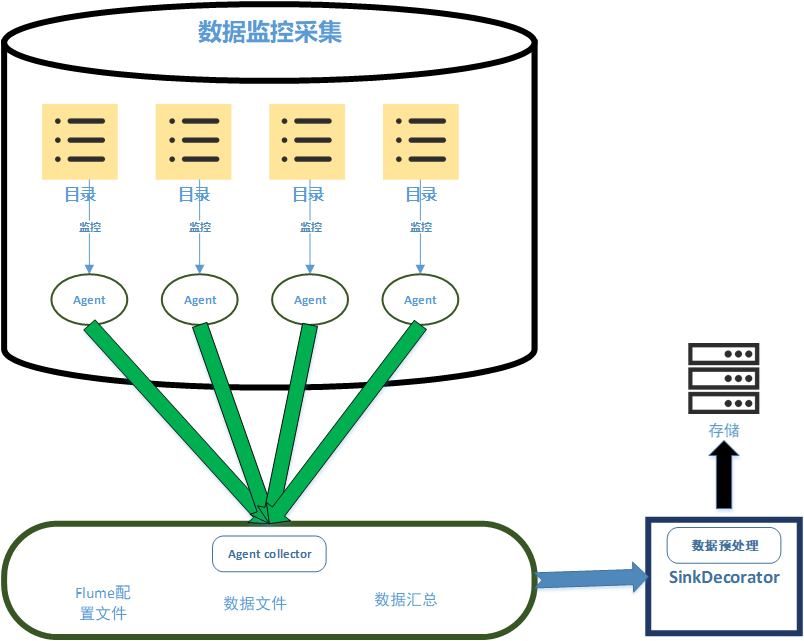
\includegraphics[scale = 0.7]{Figures/SJCJJG.png} 
    \end{generalfig}

    具体实现部分,关于Flume 的Agent配置大致如下:\\
    {\songti \bfseries \itshape
    \#对于agent中source、sinks、channels的配置\\
    a1.sources = r1\\
    a1.sinks = k1\\
    a1.channels = c1\\
    \#对于source的配置,包括类型、绑定地址、端口\\
    a1.sources.r1.type = netcat\\
    a1.sources.r1.bind = localhost\\
    a1.sources.r1.port = 44444\\
    \#对于channels的配置\\
    a1.sources.r1.channels = c1\\
    \#配置sink的类型\\
    a1.sinks.k1.type = avro\\
    \#对于sink所对应的channel的配置\\
    a1.sinks.k1.channel = c1\\
    \#配置channel的类型和容量\\
    a1.channels.c1.type = memory\\
    a1.channels.c1.capacity = 1000\\
    a1.channels.c1.transactionCapacity = 100
    }

    关于上述配置文件各行代码的意义已经写在备注中,在此不再赘述,值得一提的是flume对于每一个agent都需要进行如此繁琐的配置,实际操作时可以实现编写好批量脚本文件执行批量操作;另外由于我们要实现agent collecor ,
    因此采用avro sink组件,所以agent.sinks.k1.type 应设置为avro。

    而关于传统的采集脚本实现,也在此给出简单版本的功能实现代码:\\
    {\songti \bfseries \itshape
    from ftplib import FTP\\
    ftp = FTP()  \\
    timeout = 30  \qquad \#等待时间设置\\ 
    port = 21      \qquad \#ftp端口为21\\
    ftp.connect('xxx.xxx.xxx.xxx',port,timeout) \qquad \# 输入IP地址连接FTP服务器  \\
    ftp.login('UserName','password') \qquad \# 输入登录信息登陆  \\
    print ftp.getwelcome()  \qquad \# 打印欢迎信息   \\
    ftp.cwd('file/test')    \qquad \# 配置FTP路径\\
    dir\_list = ftp.nlst()       \qquad \# 获得目录列表  \\
    for name in dir\_list:  \\
    print(name)             \qquad \# 打印文件名字  \\
    path = 'E:/ftp/data/' + name    \qquad \# 文件保存路径  \\
    f = open(path,'wb')         \qquad \# 打开要保存文件  \\
    filename = 'PRE ' + name   \qquad \# 保存FTP文件  \\
    ftp.retrbinary(filename,f.write) \qquad \# 保存FTP上的文件  \\
    ftp.delete(name)            \qquad \# 删除FTP文件  \\
    ftp.storbinary('STOR '+filename, open(path, 'rb')) \qquad \# 上传FTP文件  \\
    ftp.quit()                  \qquad \# 退出FTP服务器  
    }
    
    通过上面简单版本的python脚本代码即可实现ftp服务器的登陆和下载保存文件操作,对应不同设备时只需要对其中部分参数进行修改即可。
     
    {\songti \bfseries-对于数据存储功能:}
    数据存储功能采用GreenPlum存储采集要求高频及海量的业务指标数据,而mysql用来存储策略、权限、日志等常用文件,GreenPlum安装配置较为繁琐,但只要按照官方文档进行安装即可;而mysql部分安装则更加简单,在此一并
    略去。但是由于上层应用对于存储数据的使用要求较高,仍需要对表格结构和字段进行详细设置,以IPTV地址池利用率表为例,表结构设置如下所示:

    \begin{generaltab}{IPTV地址池利用率表}{tab:heightweight}
		\begin{tabularx}{\textwidth}{lCCC}
			\toprule
			序号&字段名&数据类型&描述\\
            \midrule
            1&imsi&Int(2)&设备编号\\
            2&eqn&VarChar(10)&设备名称\\
            3&but&VarChar(10)&业务类型\\
            4&prvs&VarChar(10)&属地\\
            5&aln&Double(5,2)&分配地址数\\
            6&adtn&Double(5,2)&地址总数\\
            7&adat&Double(5,2)&地址分配率\\
            8&atp&Double(5,2)&今日分配峰值\\
            9&aup&Double(5,2)&今日峰值利用率\\
            10&ttup&Timestamp&今日峰值出现时间\\
            11&yap&Double(5,2)&昨日分配峰值\\
            12&yup&Double(5,2)&昨日峰值利用率\\
            13&tyup&Timestamp&昨日峰值出现时间\\
            14&hup&Double(5,2)&历史峰值利用率\\
            15&thup&Timestamp&历史峰值出现时间\\
			\bottomrule
		\end{tabularx}
    \end{generaltab}

    \subsection{数据呈现部分的设计与实现}
    \subsubsection{具体需求分析}
    本部分包含数据的呈现需求分析,正如前文所说,由于数据量过于庞大,采用传统的数据罗列和文字总结会使得使用人员过于疲劳从而无法快速了解情况,因此数据呈现部分需要具备良好的视觉呈现效果,
    使得重点突出、一目了然。对于不同类型的数据呈现的侧重点不同,表现形式应当也随之而变化,即使是不具备专业知识的人也能一眼看懂。此外,数据呈现内容应当面向各级专业人员,不同专业人员所呈现
    的内容和重点应有所区别。

    因此,数据呈现部分应该具有以下功能
    
    (1) 多种图表展示功能。针对不同类型的数据通过不同类型的图表进行数据呈现,使得呈现重点一目了然。

    (2) 针对不同维度,呈现不同的界面内容,使得各专业人员对所关心对象能够细化了解详情。

    \subsubsection{设计与实现}
    根据数据呈现功能的需求分析以及第二章中关于数据呈现技术的介绍,最终选择借助FineBI工具进行前端数据呈现,数据包与视图的关系大致如下图:

    \begin{generalfig}{数据呈现功能架构}{fig:SJCX} 
        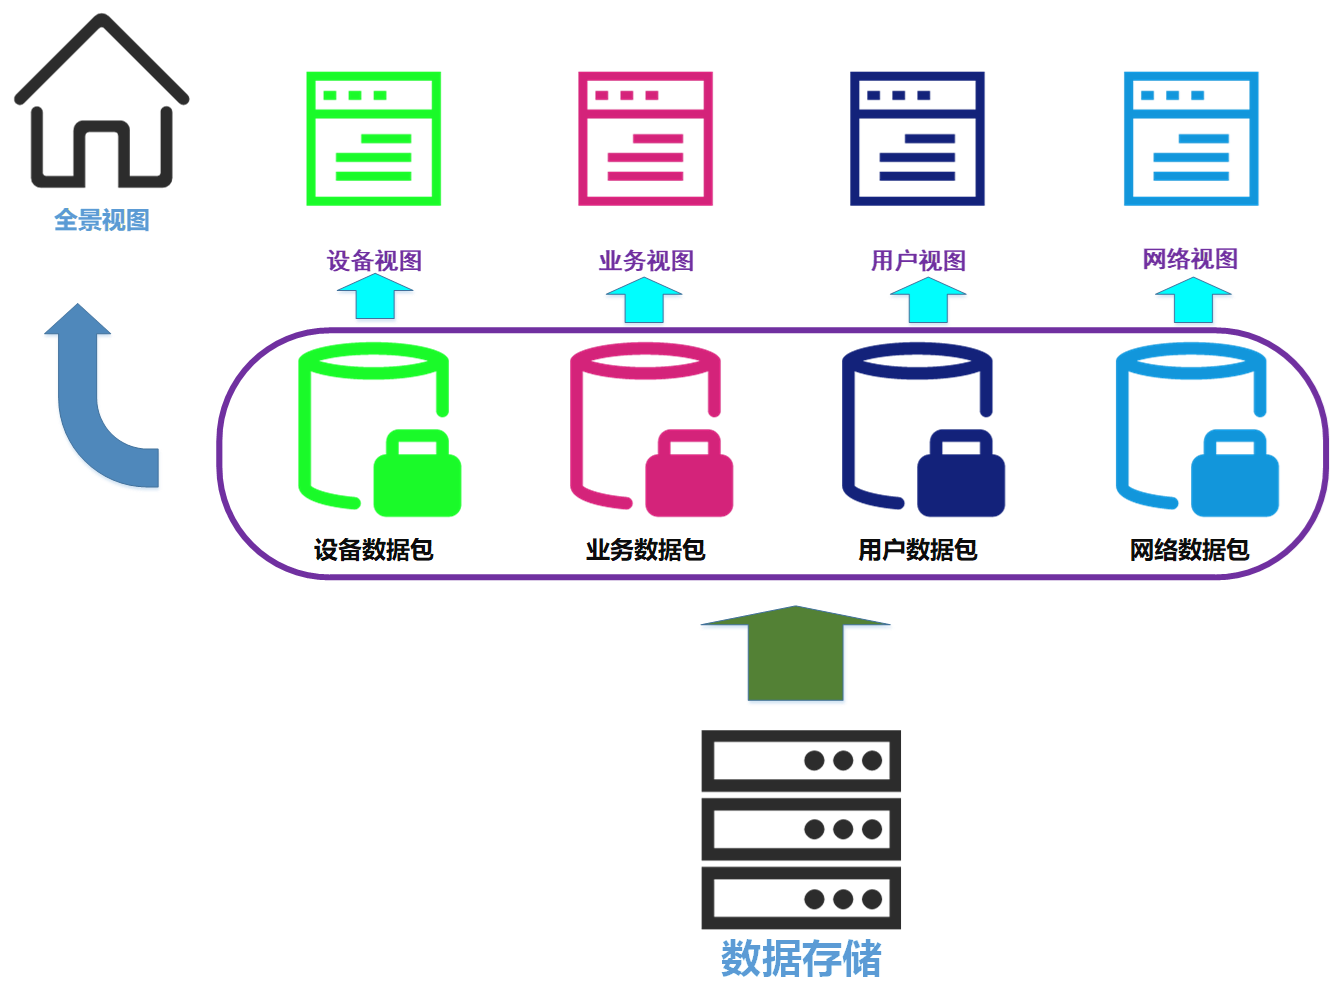
\includegraphics[width = \textwidth]{Figures/SJCX.png} 
    \end{generalfig}

    通过创建设备视图来描述,具体实现方法:\\
    1. 在数据配置面板创建新业务包,并选择类型为FineIndex。\\
    2. 在业务包中上传数据表格,并将表中外键与其他表进行关联。 \\

    \begin{generalfig}{业务包内各表关联}{fig:GBGL} 
        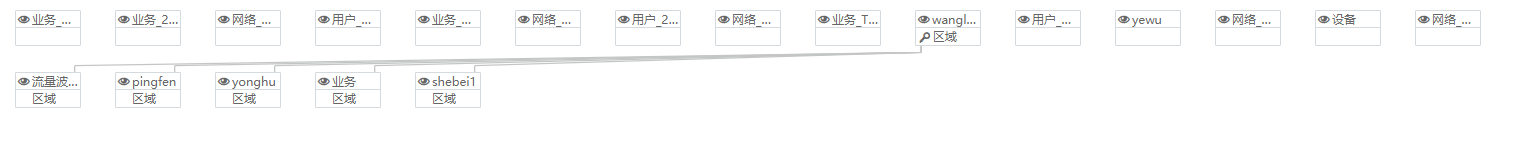
\includegraphics[width = \textwidth]{Figures/GBGL.png} 
    \end{generalfig}

    3. 对FineIndex进行更新。\\
    4. 回到仪表盘创建新的仪表盘并命名为设备视图。\\
    5. 在左侧图标栏选择合适的图表形式,并从业务包中选择数据填充。\\
    \begin{generalfig}{各种图表形式}{fig:TBXS} 
        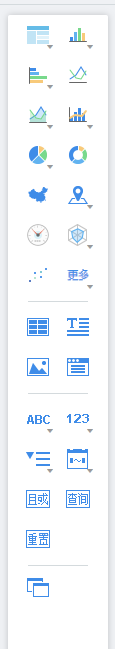
\includegraphics[scale = 0.5]{Figures/TBXS.png} 
    \end{generalfig}

    其他视图创建过程与此类似,最终完成的五大视图分别如图所示:

    \begin{generalfig}{全景视图}{fig:QJST} 
        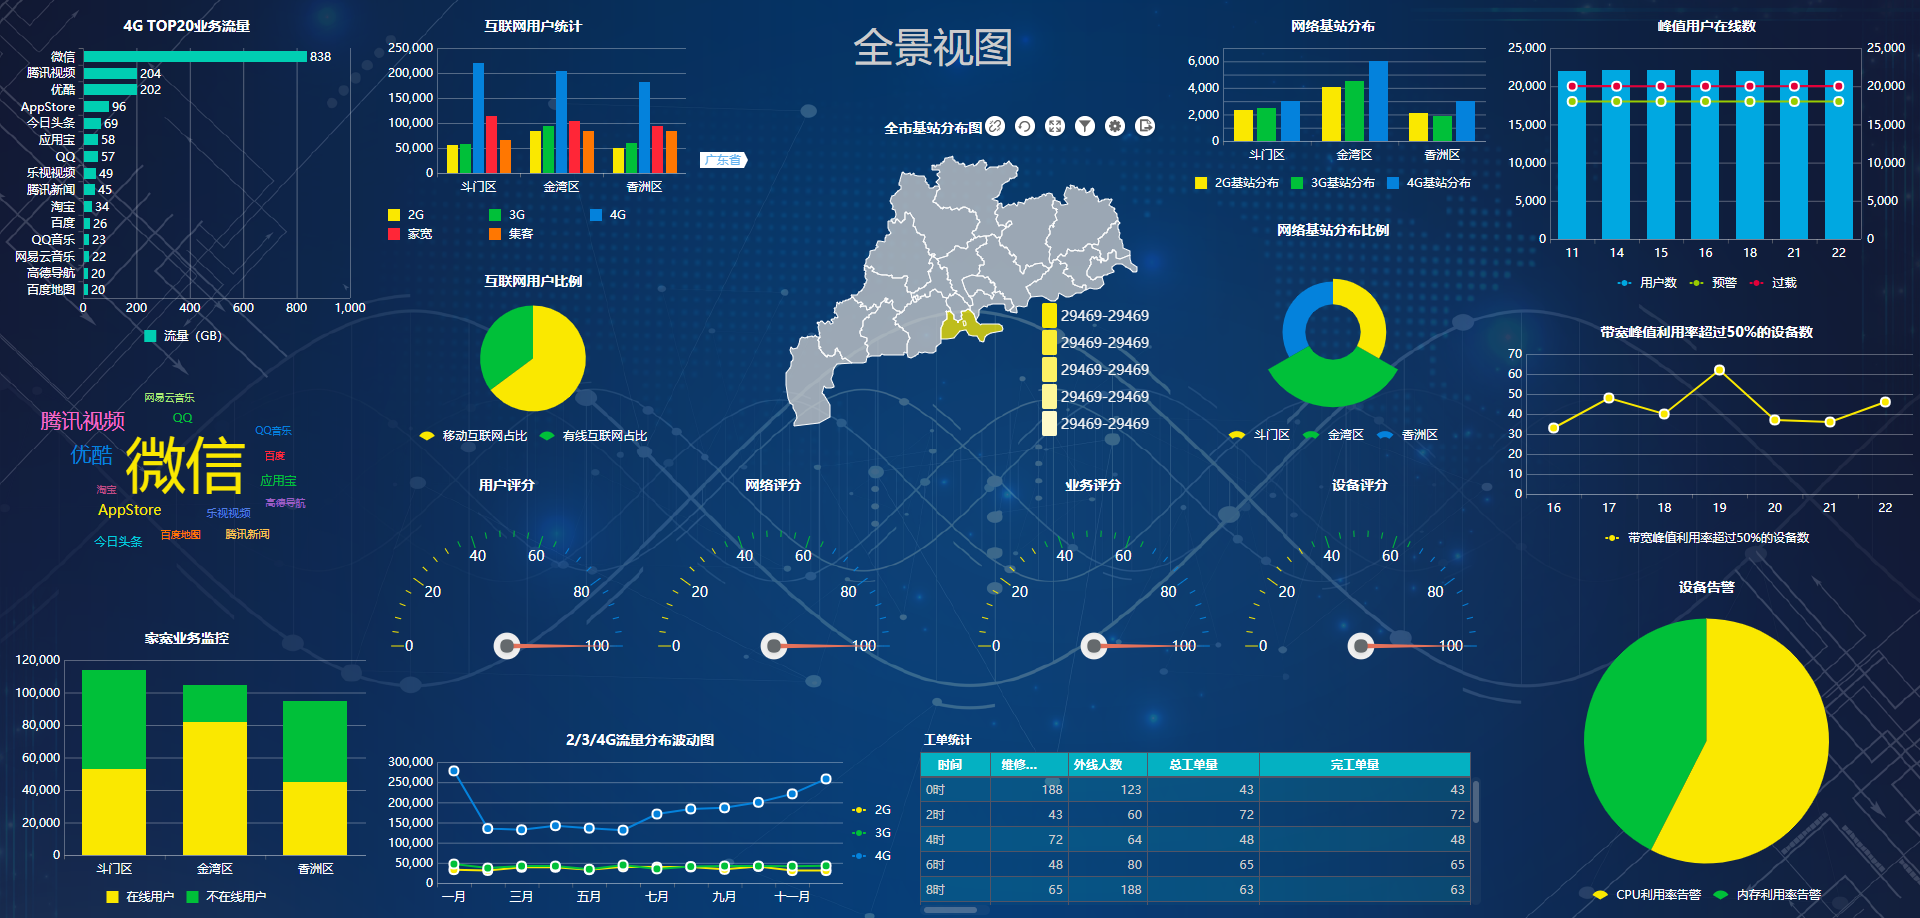
\includegraphics[width = \textwidth]{Figures/QJST.png} 
    \end{generalfig}

    \begin{generalfig}{设备视图}{fig:SBST} 
        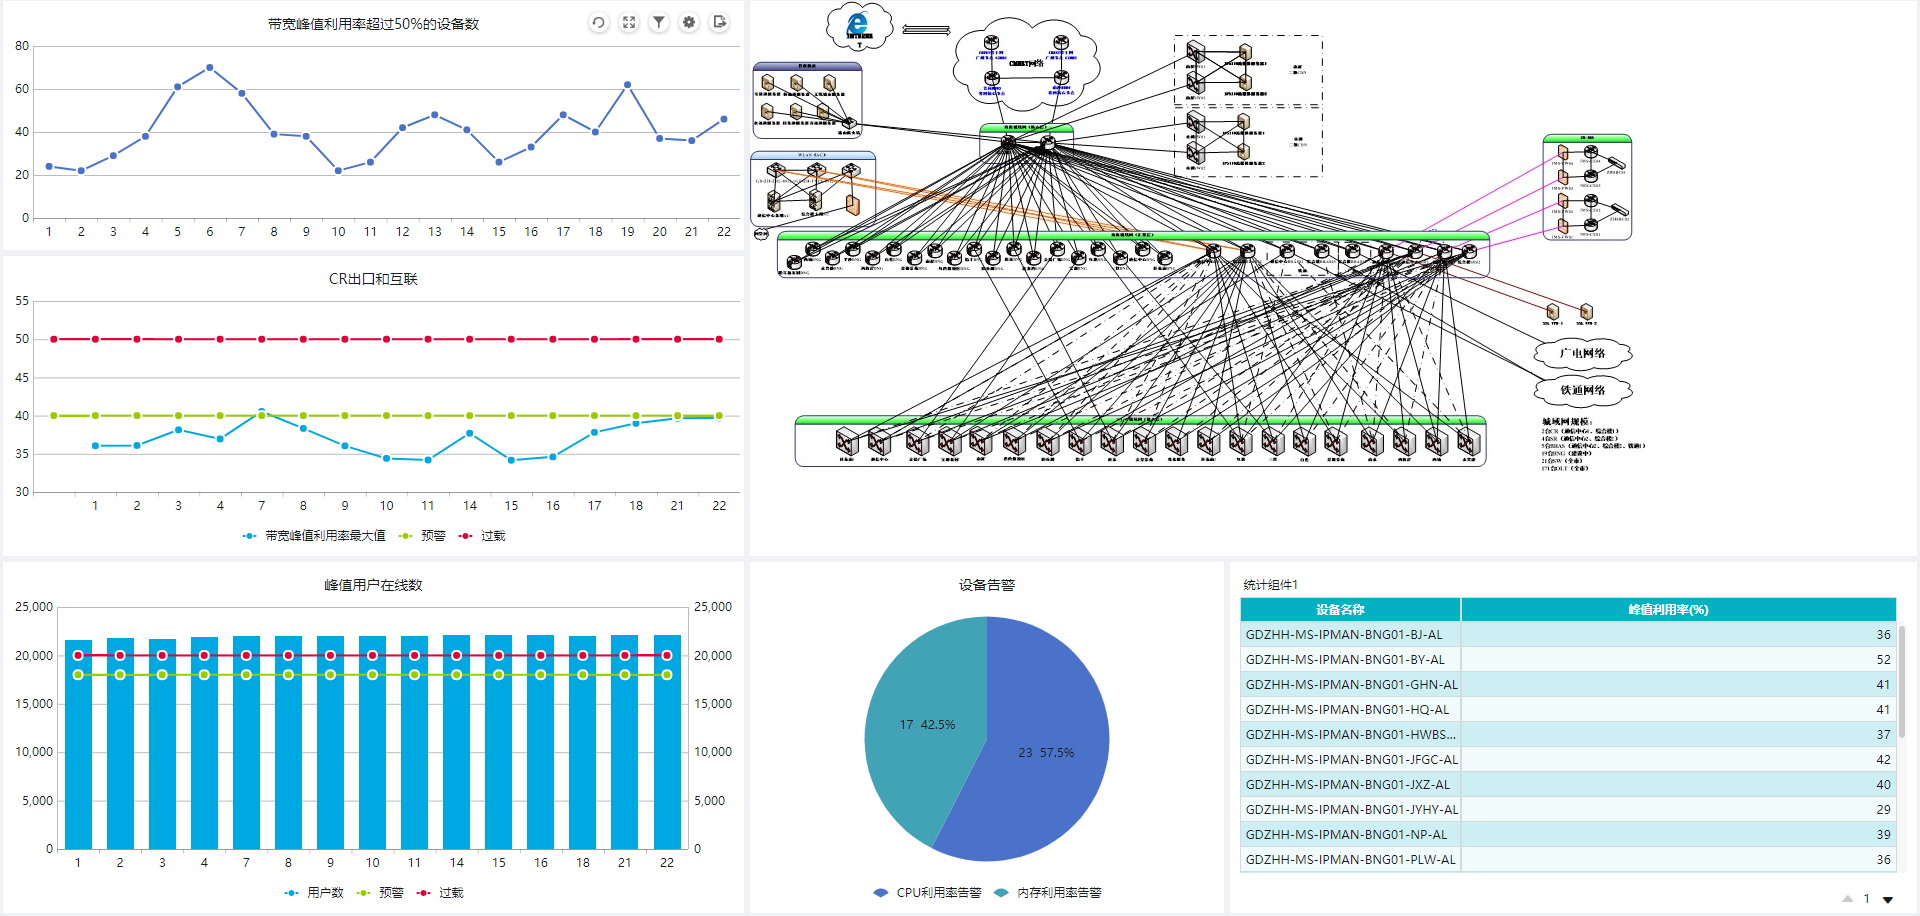
\includegraphics[width = \textwidth]{Figures/SBST.png} 
    \end{generalfig}

    \begin{generalfig}{业务试图}{fig:YWST} 
        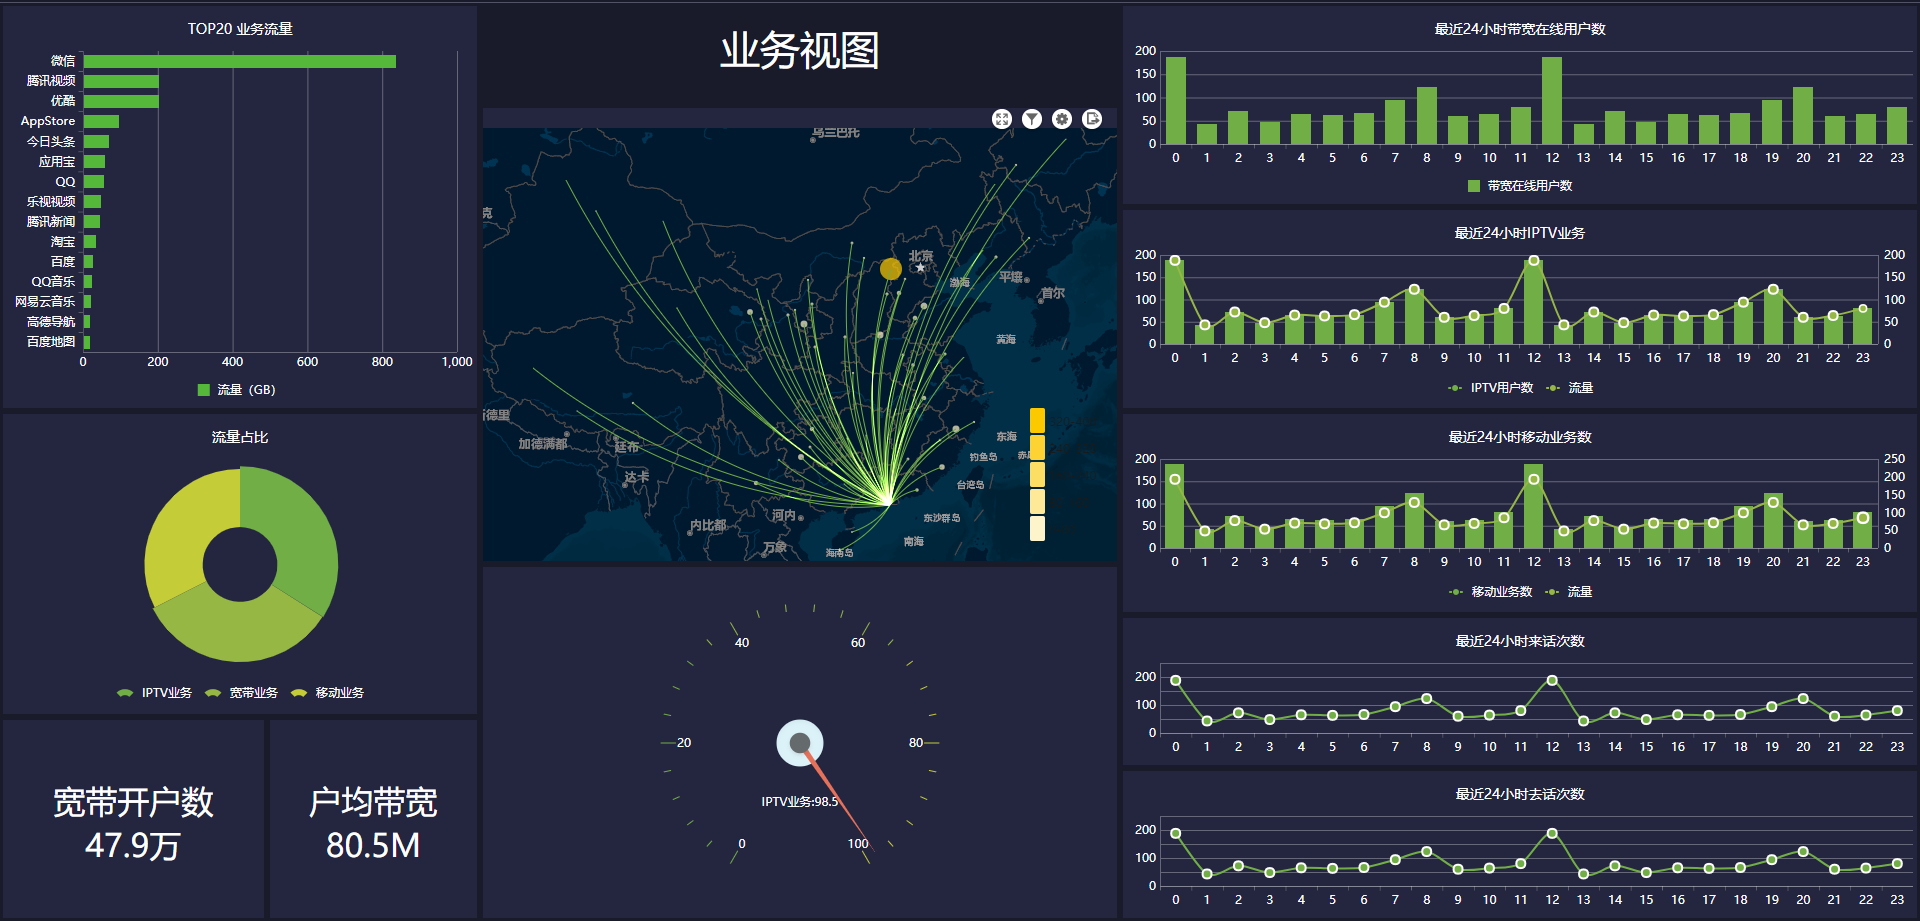
\includegraphics[width = \textwidth]{Figures/YWST.png} 
    \end{generalfig}

    \begin{generalfig}{用户视图}{fig:YHST} 
        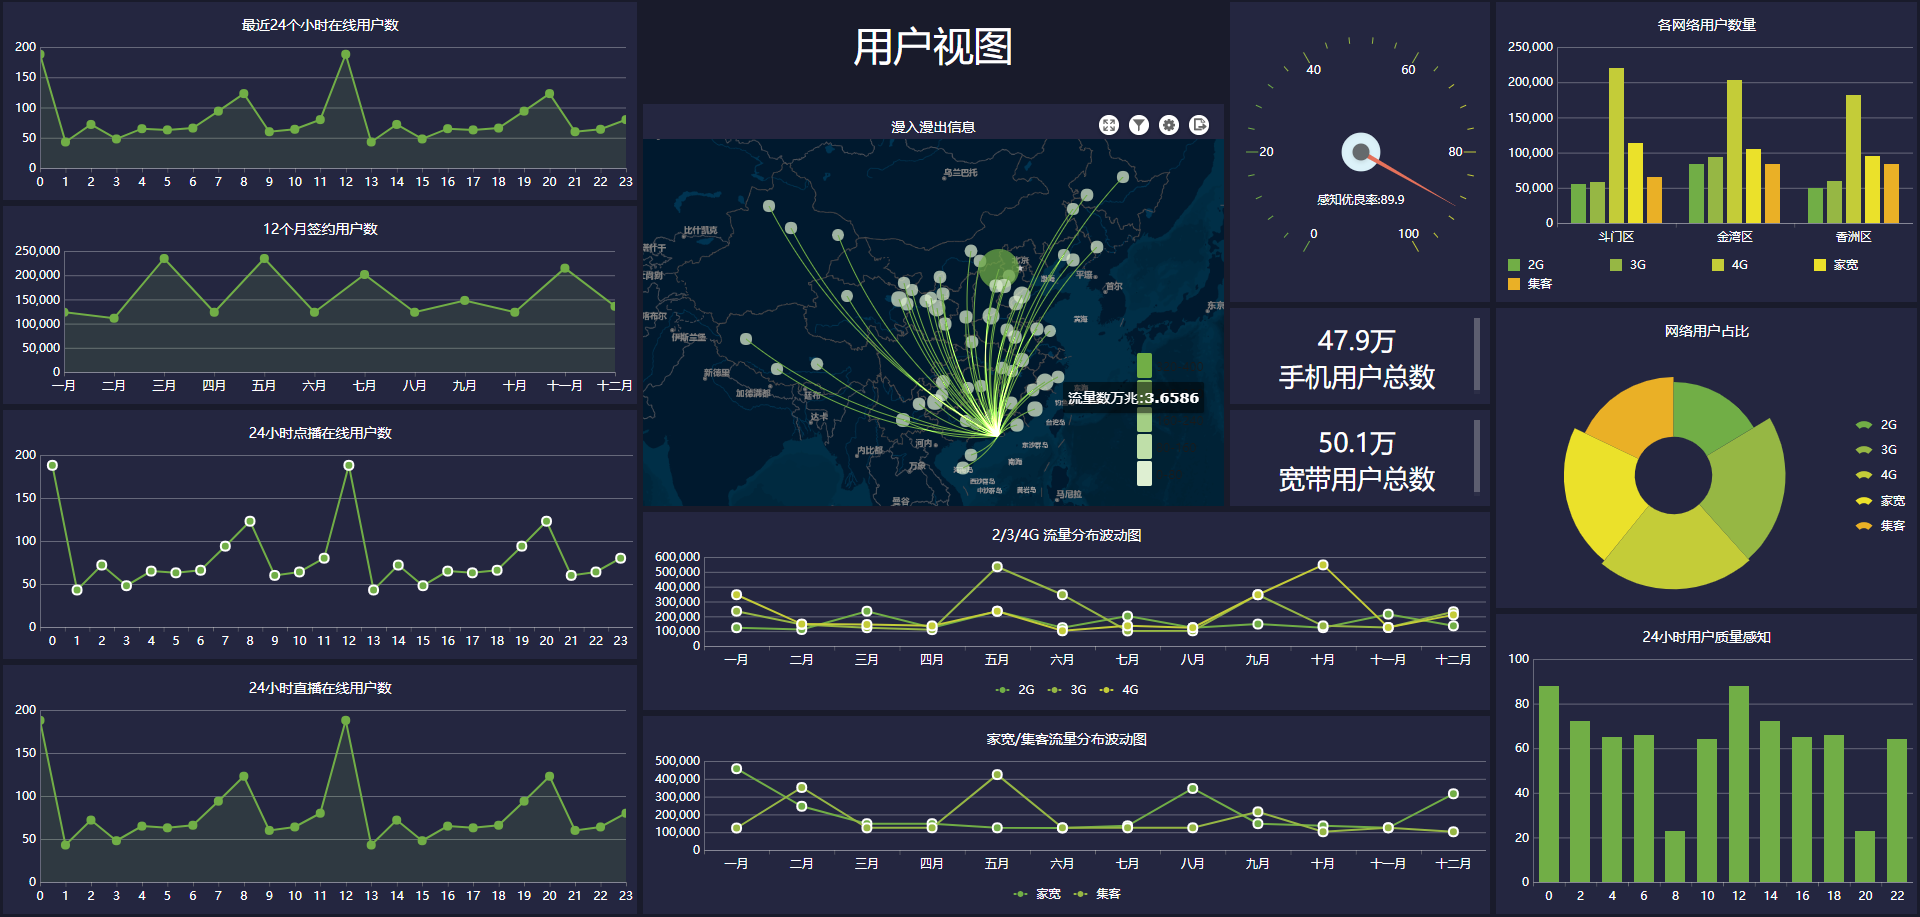
\includegraphics[width = \textwidth]{Figures/YHST.png} 
    \end{generalfig}

    \begin{generalfig}{网络视图}{fig:WLST} 
        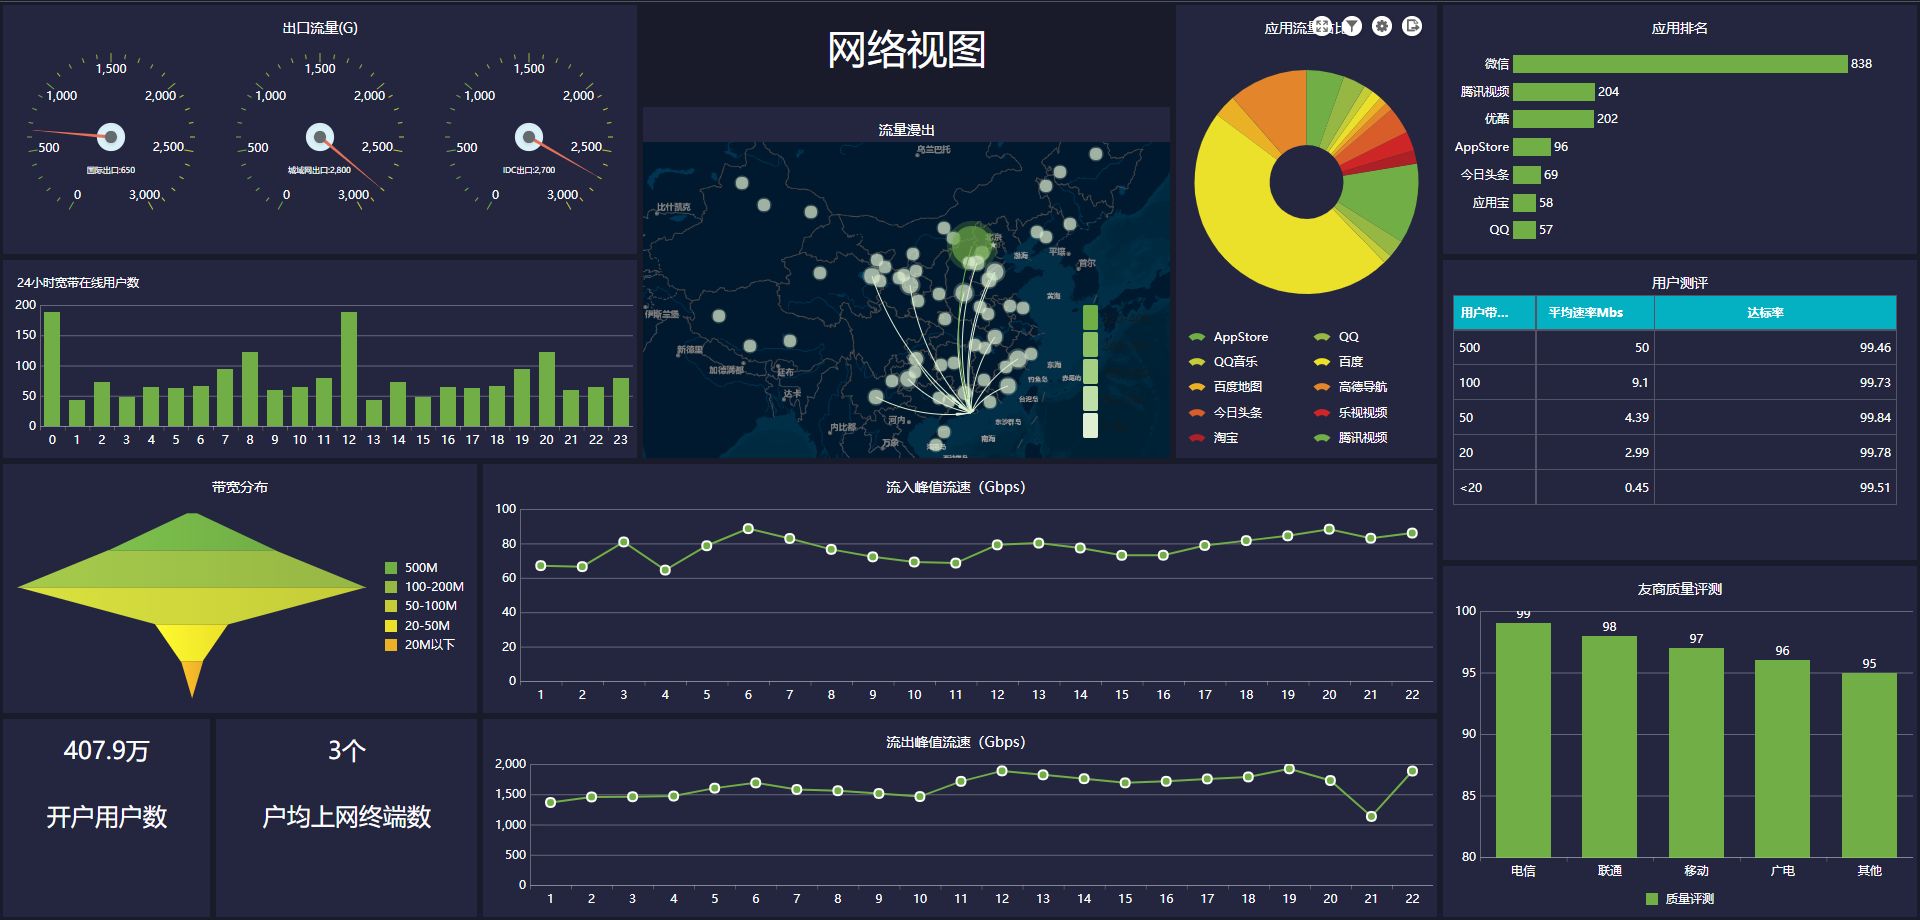
\includegraphics[width = \textwidth]{Figures/WLST.png} 
    \end{generalfig}


    \subsection{数据分析应用举例}

    这么一个运营商的用于网络管理的大数据系统的数据最终要通过上层的应用通过数据挖掘的方法来挖掘数据潜在的价值,由于数据挖掘算法大多都十分成熟,因此在实际的应用过程中只需要找到合适的场景,选定相应的
    模型即可通过数据库中的数据对模型进行训练,只要数据足够多,训练后达到一定准确率即可上线应用,在网络管理的各方面,无论是在故障定位还是投诉预测方面等都能发挥强大的力量。

    在此举一个关于异常检测的例子:\\
    {\songti \bfseries 问题描述:}在城域网维护过程中,存在着大量的KPI指标(链路利用率、端口状态、CPU利用率、内存利用率…),当这些KPI指标发生异常时,如何能够快速检测。\\
    {\songti \bfseries 输入:}一根待标注的KPI曲线和一段已经标注出的异常片段(模板)。\\
    {\songti \bfseries 输出:}KPI曲线上与模板相似的异常片段。\\

    \begin{generalfig}{异常检测}{fig:YCJC} 
        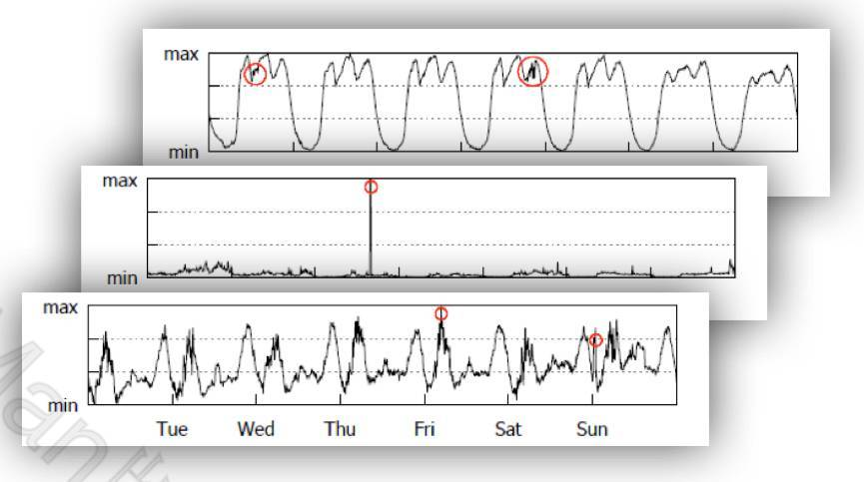
\includegraphics[width = \textwidth]{Figures/YCJC.png} 
    \end{generalfig}

    通过该问题的描述,能够得到这个问题的输入数据以及期望输出,因此由于有了大数据系统的基础支撑使得能够调用大量的过去的异常数据作为训练集,理论上是能够通过机器学习的方法训练出异常分类器来对异常的KPI进行检测。
    一种解决思路如下图所示:

    \begin{generalfig}{异常检测解决方法}{fig:JJFF} 
        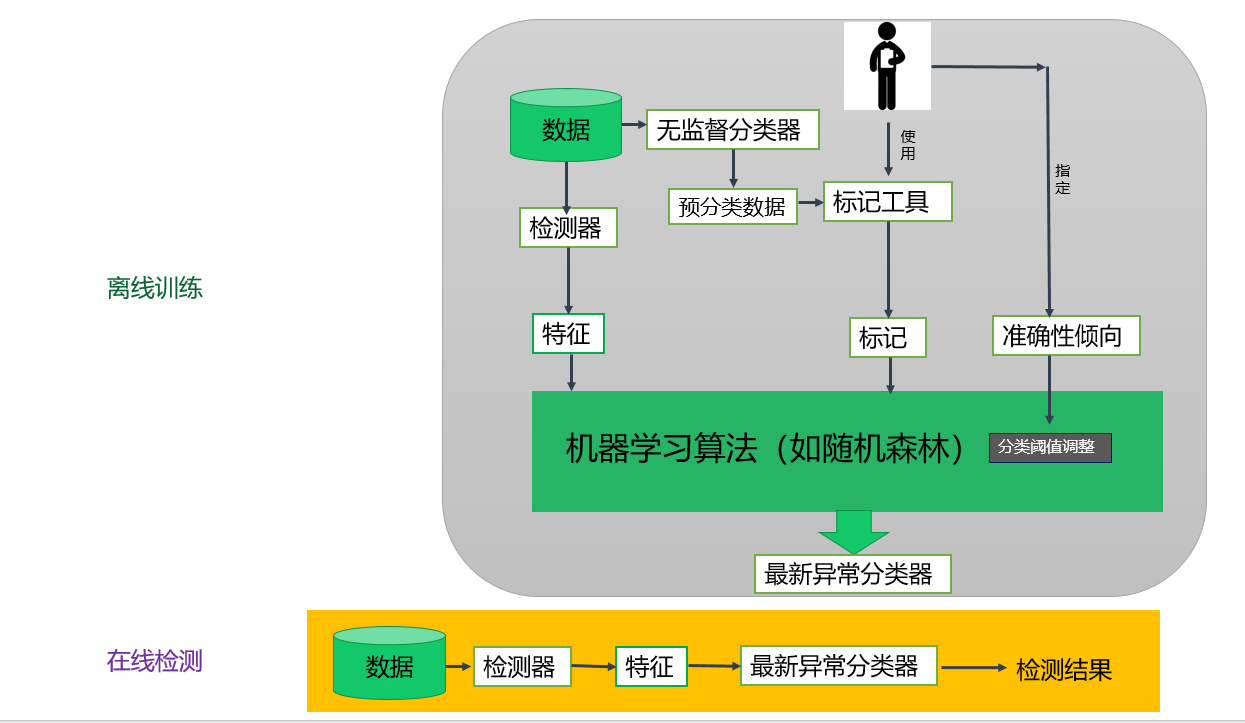
\includegraphics[width = \textwidth]{Figures/JJFF.png} 
    \end{generalfig}

    \subsection{本章小结}
    本章主要完成对于建设运营商网络管理维护大数据系统的整体架构与需求分析,并就其中部分功能的实现做了可行性验证分析。详细描述了该系统的数据采集、存储以及数据呈现部分的实现方法,通过高效、有效的方法采集、存储全网
    数据,由此支撑更高层面的数据挖掘应用;最终通过良好的数据呈现功能将数据结果进行展示,对网络运维管理的日常工作提供了便利。除此之外,还对大数据在实际的异常检测问题中的应用给出了建议和思路。
    \section{总结与展望}
    \subsection{论文工作总结}
    \subsection{未来工作展望}
    \begin{thankpage}
		
	\end{thankpage}
    
    

\end{document} 